\ifcsname pdfmapfile\endcsname
\pdfmapfile{+lm.map}
\pdfmapfile{+cm.map}
\pdfmapfile{+cmextra.map}
\pdfmapfile{+symbols.map}
\pdfmapfile{+latxfont.map}
\fi
\documentclass[aspectratio=169,11pt]{beamer}
\usepackage{booktabs,graphicx}
\usepackage[ruled,lined,shortend]{algorithm2e}
\definecolor{ink}{HTML}{17324A}
\definecolor{accent}{HTML}{166B69}
\setbeamercolor{normal text}{fg=ink,bg=white}
\setbeamercolor{frametitle}{fg=ink}
\setbeamercolor{structure}{fg=accent}
\setbeamertemplate{navigation symbols}{}
\setbeamertemplate{footline}{\hfill{\color{accent}\small\insertframenumber}\hspace{6mm}\vspace{3mm}}
\setbeamersize{text margin left=10mm,text margin right=10mm}
\setbeamertemplate{frametitle}{\vspace{3mm}\insertframetitle\par\vspace{1mm}{\color{accent}\rule{11mm}{1.1pt}}}
\newcommand{\source}[1]{\vfill{\scriptsize\color{ink!75}#1}}
\begin{document}
\begin{frame}[plain]
\begin{flushleft}
{\color{accent}Sidhant Mohanty\quad|\quad IIT Indore}\par\vspace{7mm}
{\LARGE\bfseries Batch Conformal Decision Theory\\[1.5mm]with Fewer Counterfactual Evaluations}\par\vspace{7mm}
{\large By evaluating alternative decisions on a calibration dataset, batch conformal decision theory selects a rule that controls expected loss on a new example.}
\end{flushleft}
\end{frame}
\begin{frame}{Exact calibration on a grid}
{\large\textbf{Last unsafe index}}\par
\[
 \rho_i=\max\bigl(\{j:L_i(\lambda_j)=1\}\cup\{0\}\bigr),\qquad
 \widehat\lambda=\lambda_{\rho_{(k+1)}+1}.
\]
\smallskip
\begin{tabular}{@{}ll@{}}
Calibration budget & $k=\lfloor(n+1)\alpha-1\rfloor$ unsafe examples\\
Threshold query & $L_i(\lambda_j)=\mathbf1\{\rho_i\ge j\}$\\
Anchored selection (Algorithm 1) & $O(n+\log J\log n)$ queries in expectation\\
Exact worst-case lower bound & $\Omega(n+\log J)$ for $J\ge3$, $0\le k\le n-2$\\
\end{tabular}
\source{Nonincreasing binary realized losses. Descending order statistics. Index $J+1$ denotes the safe fallback. Manuscript, Lemma 3.1 and Theorems 3.3--3.4.}
\end{frame}
\begin{frame}{Large-grid query counts}
\large Mean threshold queries per example over $40$ draws at $n=2{,}000$ and $J=8{,}193$.\par\vspace{6mm}
\centering\normalsize\renewcommand{\arraystretch}{1.5}
\begin{tabular}{@{}lrrr@{}}\toprule
Last-unsafe indices & Certified bisection & Algorithm 1 & Two-way\\\midrule
Sparse, near zero & 4.89 & 2.74 & \textbf{2.13}\\
Dense, near zero & 4.28 & 4.76 & \textbf{3.52}\\
Dense, uniform positive indices & \textbf{1.85} & 5.10 & 3.50\\\bottomrule
\end{tabular}
\par\raggedright\source{Synthetic last-unsafe indices. We use the same anchor pass when comparing the two selection variants. Manuscript, Table 2.}
\end{frame}
\begin{frame}{Joint stopping on affine solution paths}
\textbf{Independent stopping}\par\smallskip
For each example, independent stopping locates the last unsafe decision or exhausts the path before taking the batch order statistic.\par\vspace{3mm}
\textbf{Joint stopping}\par\smallskip
The joint sweep advances the path with the rightmost remaining event until $k+1$ distinct examples have produced an unsafe decision.\par\vspace{3mm}
\textbf{Graded losses}\par\smallskip
The graded sweep starts at the zero-loss fallback and updates the maximum on each path until that maximum reaches one or the path is exhausted.
\source{The sweep visits events in decreasing order until the sum of the running maxima exceeds the budget. For $M_i(\lambda)=\sup_{u\ge\lambda}L_i(u)$, a feasible deployed parameter satisfies $\sum_{i=1}^n M_i(\lambda)\le(n+1)\alpha-1$. Under exchangeability, $\mathbb E[L_{n+1}(\lambda)]\le\alpha$. Manuscript, Corollary 4.6.}
\end{frame}
\begin{frame}{Two-stage set covering with integer recourse}
\centering
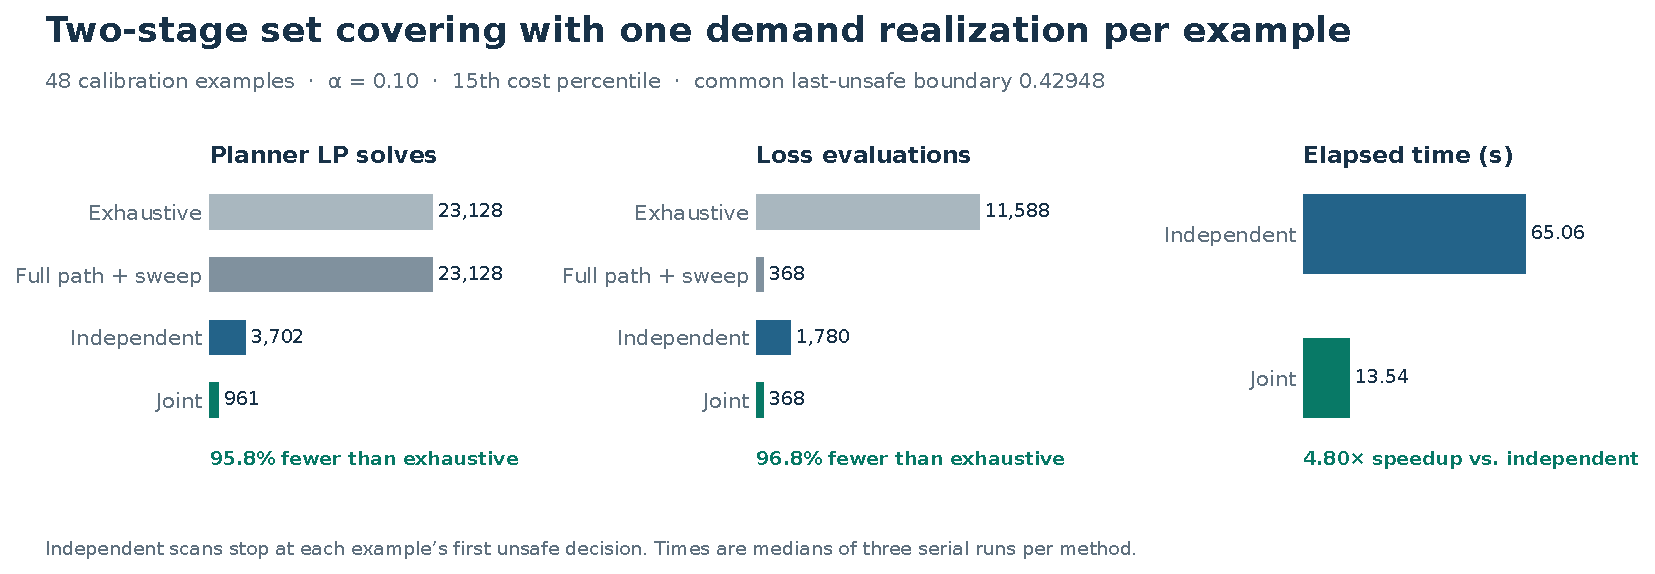
\includegraphics[width=\linewidth,height=.69\textheight,keepaspectratio]{../experiments/figures/set_cover_T1.pdf}
\par\raggedright\source{One demand realization per calibration example. The first two panels count operations. For each stopping rule, we report the median elapsed time over three serial runs in the third panel. Manuscript, Tables 3--4.}
\end{frame}
\begin{frame}{Threshold sensitivity and timing baselines}
\textbf{Across 34 set-covering settings}\par
Median reduction relative to independent stopping\par
{\large\color{accent}29.1\% fewer planner solves\qquad 30.3\% fewer loss evaluations}\par\vspace{4mm}
\textbf{At the selected thresholds}\par\smallskip
\small\renewcommand{\arraystretch}{1.32}
\begin{tabular}{@{}lrr@{}}\toprule
Baseline & One demand realization & Ten realizations\\\midrule
Independent stopping, measured end to end & $4.80\times$ & $4.41\times$\\
Full enumeration, separately timed stages & $44.5\times$ & $74.6\times$\\\bottomrule
\end{tabular}
\source{Seventeen thresholds per task on the same 48 calibration examples. We estimate the full-enumeration speedup by dividing the sum of stage times by the measured on-demand time from the same experiment. Manuscript, Section 5.3 and Appendix B.}
\end{frame}
\begin{frame}[t]
\smallskip
\begingroup
\scriptsize
\SetAlFnt{\scriptsize}
\SetAlCapFnt{\small}
\SetAlCapNameFnt{\small}
\begin{algorithm}[H]
\caption{Anchored randomized Quickselect}\label{alg:anchor-code}
\KwData{Grid $\lambda_1<\cdots<\lambda_J$, safe fallback $\lambda_{J+1}$, nonincreasing binary loss oracles $L_i$, and budget $k$. Reuse cached query answers.}
\KwResult{Calibrated cutoff $\widehat\lambda$.}
$U\gets\{i\in\{1,\ldots,n\}:L_i(\lambda_1)=1\}$\;
\lIf{$|U|\le k$}{\Return $\lambda_1$}
$r\gets k+1$\;
\While{\textnormal{true}}{
  Draw $p$ uniformly from $U$ and find $t=\rho_p$ by bisection on $\{1,\ldots,J\}$\;
  $U_{>}\gets\emptyset$, \quad $U_{=}\gets\{p\}$, \quad $U_{<}\gets\emptyset$\;
  \ForEach{$i\in U\setminus\{p\}$}{
    \lIf{$t<J$ \textnormal{and} $L_i(\lambda_{t+1})=1$}{insert $i$ into $U_{>}$}
    \lElseIf{$L_i(\lambda_t)=1$}{insert $i$ into $U_{=}$}
    \lElse{insert $i$ into $U_{<}$}
  }
  \lIf{$r\le |U_{>}|$}{$U\gets U_{>}$}
  \lElseIf{$r\le |U_{>}|+|U_{=}|$}{\Return $\lambda_{t+1}$}
  \lElse{$r\gets r-|U_{>}|-|U_{=}|$,\quad $U\gets U_{<}$}
}
\end{algorithm}
\endgroup
\end{frame}

\begin{frame}[t]
\smallskip
\begingroup
\scriptsize
\SetAlFnt{\scriptsize}
\SetAlCapFnt{\small}
\SetAlCapNameFnt{\small}
\begin{algorithm}[H]
\caption{Backward event sweep}\label{alg:sweep-code}
\KwData{For each example $i$, a right-to-left stream of winning intervals and singleton tie events, with binary loss $\ell_i(E)$ and right endpoint $r(E)=\sup E$ for each event $E$; budget $k$.}
\KwResult{Batch last-unsafe boundary $V_{(k+1)}$.}
$H\gets$ empty max-heap keyed by $r(E)$,\quad $c\gets 0$\;
\ForEach{$i\in\{1,\ldots,n\}$}{
  Take the first event $E$ from stream $i$ and push $(r(E),i,E)$ into $H$\;
}
\While{$H\ne\emptyset$}{
  $(r,i,E)\gets\operatorname{popMax}(H)$\;
  \eIf{$\ell_i(E)=1$}{
    $V_i\gets r$,\quad $c\gets c+1$\;
    \lIf{$c=k+1$}{\Return $r$}
  }{
    \If{stream $i$ has another event $E'$}{
      Take $E'$ and push $(r(E'),i,E')$ into $H$\;
    }
  }
}
\Return $-\infty$\;
\end{algorithm}
\endgroup
\end{frame}
\end{document}
